\documentclass[tikz]{standalone}

\usetikzlibrary{arrows.meta}
\usetikzlibrary{positioning}
\usetikzlibrary{external}

\begin{document}
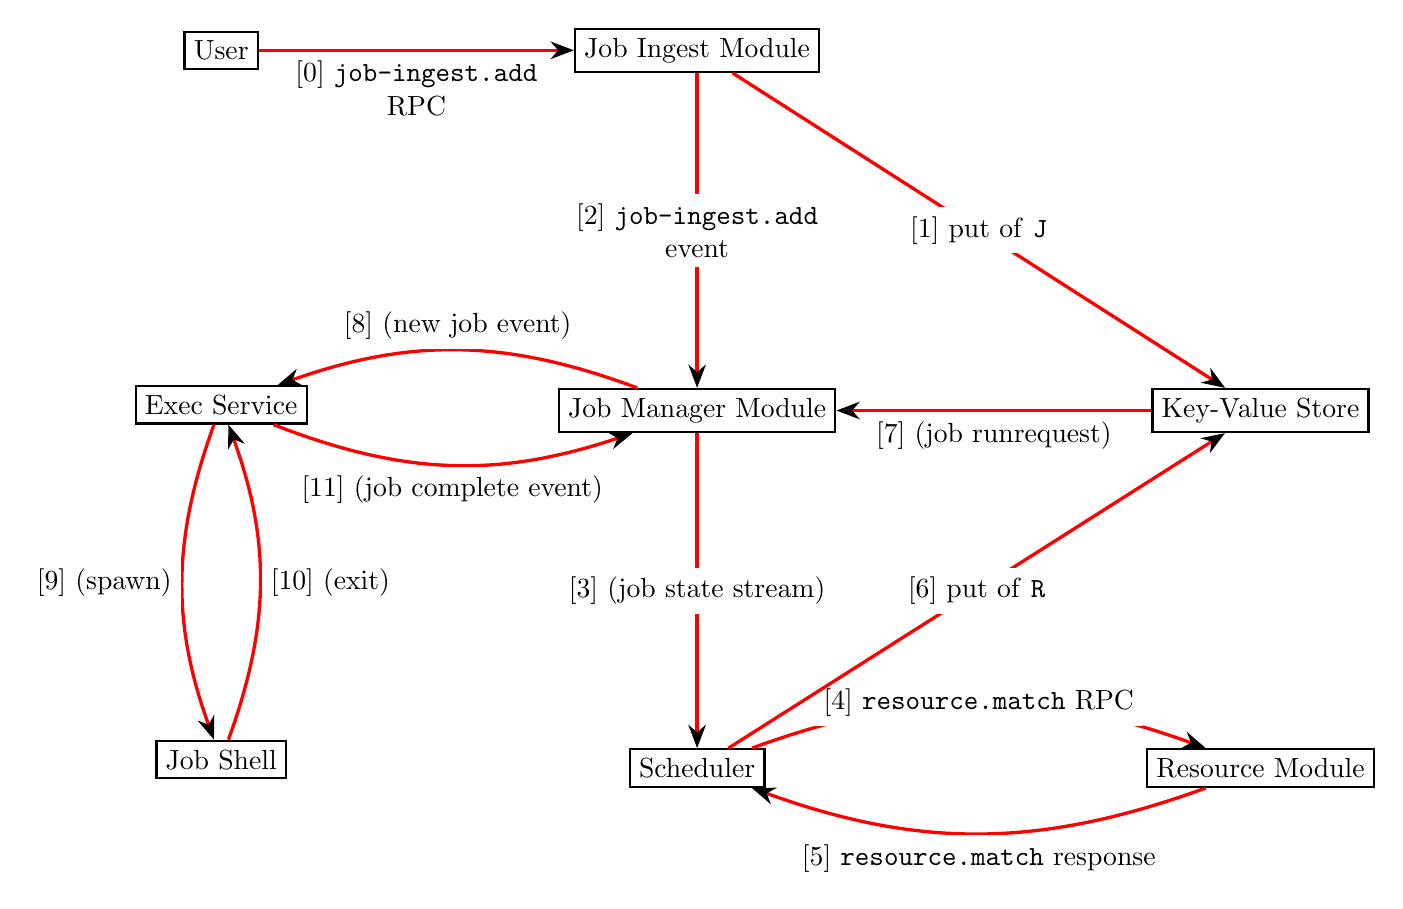
\begin{tikzpicture}
\begin{scope}[every node/.style={thick,draw,rectangle}]
    \node (user) at (0,0)                   {User};
    \node[right=4 of {user}]    (ingest)    {Job Ingest Module};
    \node[below=4 of {ingest}]  (job_man)   {Job Manager Module};
    \node[below=4 of {job_man}] (sched)     {Scheduler};
    \node[right=4 of {job_man}] (kvs)       {Key-Value Store};
    \node[below=4 of {kvs}]     (res)       {Resource Module};
    \node[below=4 of {user}]    (exec)      {Exec Service};
    \node[below=4 of {exec}]    (job_shell) {Job Shell};
\end{scope}

\newcounter{MajorEventCount}
\newcommand{\newEvent}{\arabic{MajorEventCount}\stepcounter{MajorEventCount}}

\begin{scope}[>={Stealth[black]},
              every node/.style={fill=white},
              every edge/.style={draw=red,very thick,align=center}]
    \path [->] (user)      edge                node[below] {[\newEvent] \texttt{job-ingest.add} \\ RPC}  (ingest);
    \path [->] (ingest)    edge                node        {[\newEvent] put of \texttt{J}} (kvs);
    \path [->] (ingest)    edge                node        {[\newEvent] \texttt{job-ingest.add} \\ event} (job_man);
    \path [->] (job_man)   edge                node        {[\newEvent] (job state stream)} (sched);
    \path [->] (sched)     edge[bend left=20]  node        {[\newEvent] \texttt{resource.match} RPC} (res);
    \path [->] (res)       edge[bend left=20]  node[below] {[\newEvent] \texttt{resource.match} response} (sched);
    \path [->] (sched)     edge                node        {[\newEvent] put of \texttt{R}} (kvs);
    \path [->] (kvs)       edge                node[below] {[\newEvent] (job runrequest)} (job_man);
    \path [->] (job_man)   edge[bend right=20] node[above] {[\newEvent] (new job event)} (exec);
    \path [->] (exec)      edge[bend right=20] node[left]  {[\newEvent] (spawn)}  (job_shell);
    \path [->] (job_shell) edge[bend right=20] node[right] {[\newEvent] (exit)}  (exec);
    \path [->] (exec)      edge[bend right=20] node[below] {[\newEvent] (job complete event)}  (job_man);
\end{scope}
\end{tikzpicture}
\end{document}

%%% Local Variables:
%%% mode: latex
%%% TeX-master: t
%%% End:
